In this section, the outcomes obtained from examining the academic studies on Android application development are presented. Considering the tight relationship between the topic and industry, a Systematic Literature Review (SLR) was not adequate for finding relevant resources of data for the study. Hence, a Multivocal Literature Review (MLR) was conducted. As a type of SLR, MLR is collecting grey literature as well alongside formal literature \cite{40}. MLR considers resources like blogs, white papers, articles, academic literature and allows gathering information from academics, developers, practitioners, and independent researchers \cite{41}. For a topic closely related to the industrial trends, adding grey literature next to the white literature as a part of the literature review was crucial. Because the most up-to-date resources are the grey literature resources in the Android environment and to compare the white literature's situation to the latest industrial trends of the Android application development, grey literature is definitely needed. Regardless of the direct relevance of the studies to maintainability, the following research query has been used to determine all the studies related to Android application development published in the last five years. Among the determined studies, those related to maintainability have been examined in more detail. 
\begin{figure}[ht!]
    \centering
    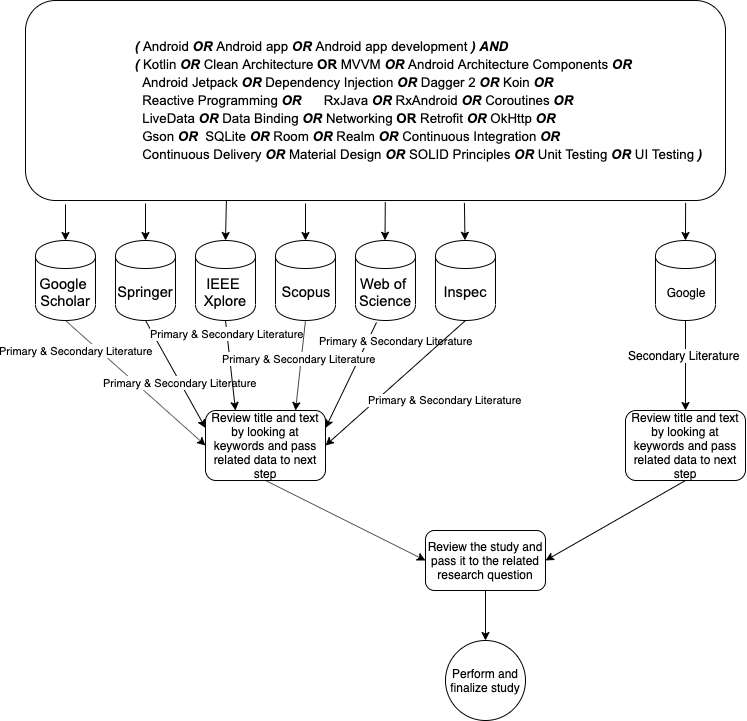
\includegraphics[scale=0.4]{figures/research_query.png}
    \caption{Search process visualization}
    \label{fig:lit_review_research_query}
\end{figure}

As a result of the executed research query above, more than forty seven papers were found and reviewed. Grey literature results are not included in these numbers. The found and reviewed grey literature results were only used to compare the academic literature and industry's situation and interpret the situation. Also, the reviewed grey literature was cited in this study. For the purpose of obtaining more successful findings, the search query was separated into six parts, each of them individually focusing on a single topic. The literature found as a result of this query was read thoroughly. Finally, inclusion and exclusion criteria were applied to the primary studies to have suitable literature only. As soon as the early research outcomes were collected, chasing the inclusion and exclusion criteria shown in Figure 6, the unrelated material was filtered out. Also, the studies conducted before 2015 are excluded from the query results to prevent any possible up-to-dateness issues.
\begin{figure}[ht!]
    \centering
    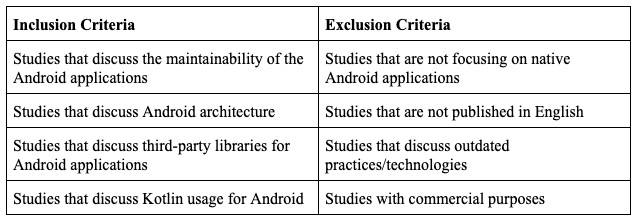
\includegraphics[scale=0.6]{figures/research_query_criteria.png}
    \caption{Inclusion and exclusion criteria}
    \label{fig:lit_review_research_query_criteria}
\end{figure}

These more than forty academic studies examined on Android application development can be grouped according to their topic titles as follows.
\begin{itemize}
    \item 4 studies bachelor theses regarding Android application development.
    \item 5 papers were related to 3rd party Android libraries.
    \item 5 papers were related to Kotlin programming language usage for Android.
    \item 5 papers were related to maintainability of the Android applications.
    \item 12 papers were related to Android app architecture.
    \item 16 papers were related to Android application development but not directly related to the topic that this study covers.
\end{itemize}

In addition to the papers mentioned above, 15 other papers are reviewed to get a better understanding of the studies conducted regarding software maintainability, metrics that can be used to measure software maintainability, general software engineering principles such as separation of concerns, and SOLID. These articles and books have been cited in various parts of this study.

Among these more than forty academic studies on Android application development that are reviewed as a part of this study, the studies on Android application architecture and maintainability draw attention. Studies conducted on these two subjects account for more than one-third of the total studies examined. Based on these numbers, it can be said that the Android application architecture and the importance of maintainability are recognized by the researchers working in the Android field. As stated in the 2.3 and 2.6 sections of this study, the importance of application architecture and maintainability in the context of Android application development processes is supported by the above numbers and academic studies included in these numbers. In most of these studies, it is noteworthy that comparisons of Android application architectures in terms of performance, maintainability, and testability are common. As mentioned in previous chapters, considering the impact of software architecture on maintainability and the importance of maintainability in software development processes, it is not surprising that many academic studies have focused on architecture and maintainability. Various studies on the maintainability of Android applications draw attention. For example, Hugo Källstrom conducted a study on a similar topic in which he implemented three different software architectures and evaluated the maintainability based on these architectures \cite{18}. Also, Prabowo et al. have a research on the maintainability of Android applications which they compared MVP and anti-pattern approaches \cite{19}. Apart from these works, the work of Verdecchia et al. (2019) on architectural choices in Android applications is a worth reading work on both architecture and maintainability topics \cite{14}. These studies regarding the architecture and maintainability in Android application development stand out as resources worth examining. There are also some other studies that are cited in the paper, they are worth reading too. On the other hand, there are some significant issues with most academic studies regarding the topic. 

First of all, it is noteworthy that academic studies in this field are inadequate. Even as a result of a comprehensive literature review that included the grey literature, around fifty studies were reached, and this number is the total number of studies on Android development. The number of studies on the maintainability of Android applications is slightly less than one-third of this total number. As explained in the previous sections, considering the importance of maintainability in Android application development, it will be seen that the number of studies in this field is insufficient. 

In addition to this quantitative problem, it is seen that there are some qualitative problems among the existing academic studies as well. As a result of the research among academic studies regarding Android application development, the conclusion is that the inadequacy of the formal resources in terms of up-to-dateness constitutes a major issue. Considering the dates of the studies and the continuous and rapid development of the Android world and the changing trends, this result is not unexpected but still points to an issue. That situation creates one of this study's motivations, which is closing this gap between industry and academia. When the literature review results are evaluated in terms of maintainability, which is the main element of this study, some significant issues are observed. 

When the studies on the maintainability of Android applications are examined, we see that many studies approach maintainability in terms of software architecture. As mentioned earlier in this study, it can be said that this result is not a surprise, considering that software architecture is one of the most significant factors in the impact on maintainability. Both academic resources and information gathered from the industry indicate that, when it comes to building Android applications with high maintainability, the architectural choices are shaped around the same main architectural and design patterns. Those can be named as MVC, MVP, MVVM and Clean Architecture. However, When the existing studies are examined, most of the studies cover the basic implementation of these design patterns and comparisons between these design patterns in terms of performance and maintainability. 
\begin{figure}[ht!]
    \centering
    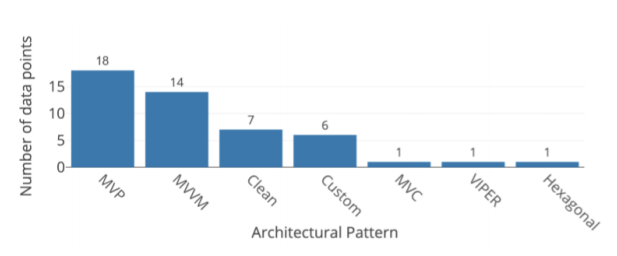
\includegraphics[scale=0.5]{figures/pattern_usage.png}
    \caption{Well-known architectural and design patterns for Android \protect\cite{14}}
    \label{fig:arch_patterns}
\end{figure}

On the other hand, considering the other factors affecting the maintainability of Android applications and some of the outdated techniques and technologies used in the studies mentioned above, it is possible to talk about the insufficiency of these studies on Android application development in the last five years. The systematic review indicates that the lack of detail and outdatedness in these studies is apparent. Another problem that strikes the eye among the academic studies reviewed is that most studies only approach the maintainability of Android applications from an architectural perspective. It is possible that other techniques and technologies can be used to increase the maintainability of Android applications besides architectural patterns. The fact that the studies do not focus on these techniques and technologies can be considered a deficiency of the academic literature regarding this topic.

In addition to the above-mentioned situation, in almost all of the examined academic studies and the reviewed work from the industry, the fact that these design patterns are presentational design patterns and they are not architectural patterns is completely ignored. In other means, the patterns derived from the MV-I concept, such as MVVM, MVP, MVC, are actually designed for how data is managed for display purposes. MV-I design patterns are intended to control the communication between the view layer and the data layer of GUI heavy applications. However, while developing small-sized Android applications, these design patterns can be effective up to a point. Nevertheless, while developing enterprise Android applications that have more sophisticated and complex business logic, it is obvious that these design patterns will be insufficient in scaling the application and solving the maintainability problems we have mentioned. Hence, the visibility of the need for higher-level architecture and other techniques when developing complex Android applications is clear.  Also, considering the study topic's tight relation with the industry, knowing the technologies, techniques, and latest trends used in the industry is also essential for studies on this subject. However, when current studies are examined, it will be seen that there are problems related to these situations.

The literature review shows that the academia lacks awareness of the industry trends and comprehensive information about techniques and technologies that can be used to develop maintainable Android applications with up-to-date tools. This study aims to fill this gap in the academia by explaining and analyzing one of the top mobile application development companies' methodologies in the region.